\chapter{Architecture/Model}
\label{sec:architectureAndModel}
This chapter contains the architecture and model of the system, which tools and methods that has been used and how they all connect together to produce the result.
An overview of the system is presented in chapter \ref{sec:overview}. A description of the robot is presented in section \ref{sec:robot}. Section \ref{sec:scenario} contains the different scenarios used in the experiment.

\begin{figure}[h]
\label{fig:overview}
\begin{center}
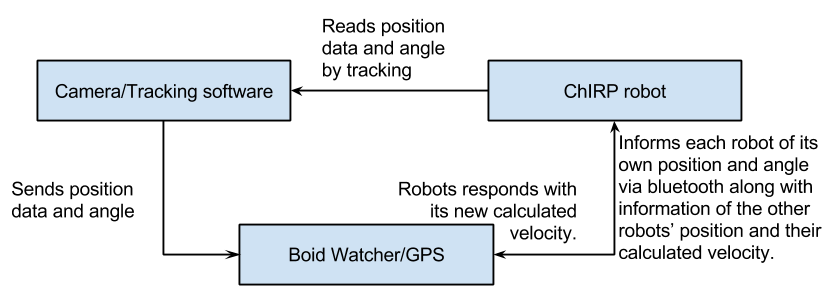
\includegraphics[width=\linewidth]{figs/system_overview}
\end{center}
\caption[System overview]{Overview of the components of the system}
\end{figure}

\section{System overview}
\label{sec:overview}
The system consists of three primary components as illustrated in Figure \ref{fig:overview}. The camera and the tracking software, the Boid-watcher which acts as a GPS and the ChIRP robots.
The camera tracking software tracks each robot's position and its angle, which is sent to the Boid-watcher. The Boid-watcher not only work as a GPS but is also the bridge between the robots, it provides information about the position and velocity of each robot to all the other robots.
Even if it is possible for one computer to run both the camera tracking, two different computers were used in this setup. The camera tracking software being run on a stationary desktop computer, and the camera is attached to a pole above a sandbox where the robots roam around. The simulator is run on a different computer, because it needs to communicate with all the robots simultaneously. The desktop computer was not able to process both the camera tracking software and the watcher GPS software while sending bluetooth data to four of the robots. Which lead to the camera not being able to update fast enough and thus crashed quite so often.
%TODO GPS

\section{Robots}
\label{sec:robot}
\begin{figure}[h]
\label{fig:robot}
\begin{center}
%TODO robot figure
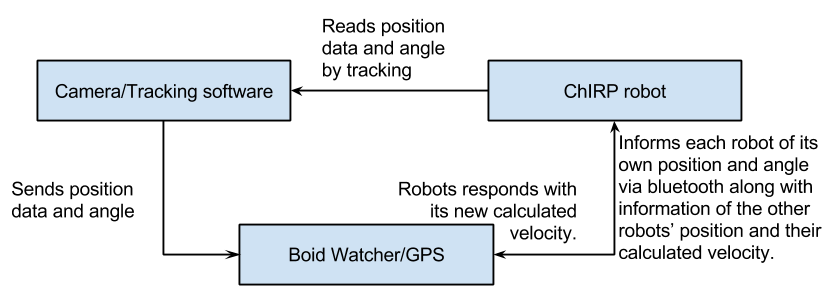
\includegraphics[width=0.8\linewidth]{figs/system_overview}
\end{center}
\end{figure}

The robot swarm consist of four ChIRP robots. The ChIRP robot is a circular shaped robot with differential wheel. A differential wheeled robot is a robot with two separate driven wheels on each side, which it can use move. If it wants to change its direction it can vary the relative speed of each wheel/motor. For instance if the right wheel moves faster than the left one, the robot will turn to its left. The advantage of differential wheel is that an additional steering motor is not required for the robot to move around.
Each robot is equipped with eight infrared LED lights and receivers used for measuring distance. The distance sensors are spaced evenly around the robot, where one of the sensors are directly in front of the robot. This sensor can be used to detect whether there is an obstacle directly in front of the robot or not.
Each of the ChIRP robot is equipped with a bluetooth module, which it uses to communicate with the watcher/GPS computer wirelessly. 
The robots are very hollow on top as seen in Figure \ref{fig:robot}, and the distance sensors have difficulties sensing other robots due to the hollowness.


\section{Scenarios}
%\begin{figure}[h]
%\label{fig:scenario0}
%\begin{center}
%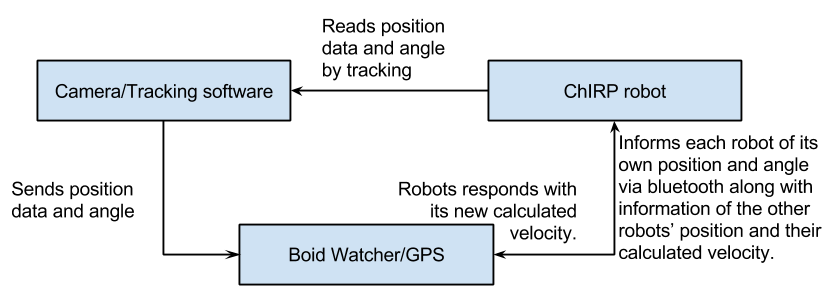
\includegraphics[width=0.8\linewidth]{figs/system_overview}
%\end{center}
%\end{figure}
\label{sec:scenario}


\section{Robot controller}
When the robot first is turned on and a bluetooth device is paired with its bluetooth module the robot will stand still and wait. The robot will wait for a command to move, turn or stop. This is when a person can manually control the robot. If the watcher sends data to the robot, it will start to calculate where it should go based on the data it received. 
%TODO
It will then check the whether there is an obstacle in front of it, then rotate if there is one. 
When the robot has calculated which direction it wants to go, it will find out which direction it needs to face and turn itself approximately in that direction. The robot will then measure the distances in case it has turned towards an obstacle. If there is no obstacle in front of it, it will move forward and wait for new data from the watcher software. If the robot did find an obstacle in front of it, it will turn 90\textdegree. The robot will stop after turning and wait for new data from the watcher software. 
\begin{figure}[h]
\label{fig:robotschema}
\begin{center}
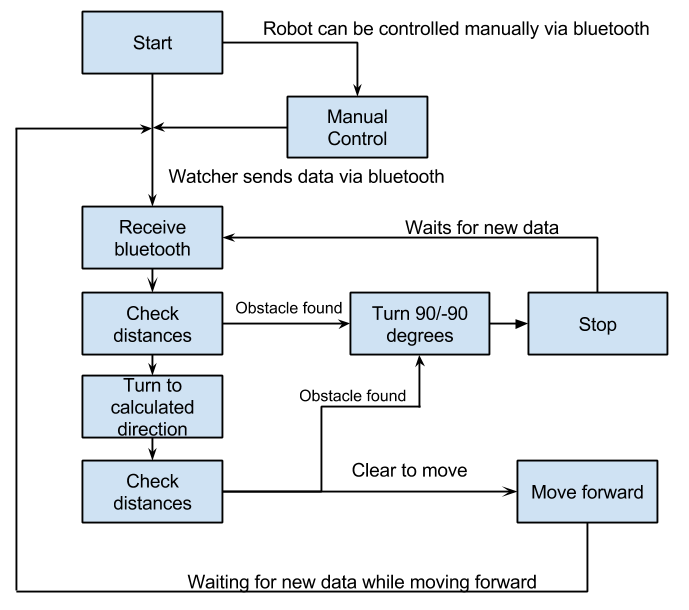
\includegraphics[width=0.8\linewidth]{figs/robotschema}
\end{center}
\caption[Robot flowchart]{Flowchart of the robot}
\end{figure}

\section{Simulator}

A simulator was created where the Boids was implemented solely in software and rendered on screen, that is no physical robots were used in the simulator. The reason to use a simulator was to see how the Boids were supposed to behave and have a working example to compare with.

\section{Differences between physical and simulator}
The physical robots are trying to mimic the behavior of the Boids created in the simulator. However a physical robot is different than the Boids created in the simulator by nature. As discussed in section \ref{sec:robot}, the robots are a type of differential wheeled robots, which means that it can only move forward or backwards, turn on the spot or move and turn at the same time. The Boids in simulator software did not have any direction, they were able to move freely in all 360\textdegree direction.